\documentclass[11pt,a4paper]{report}
\usepackage[textwidth=37em,vmargin=30mm]{geometry}
\usepackage{calc,xunicode,amsmath,amssymb,paralist,enumitem,tabu,booktabs,datetime2,xeCJK,xeCJKfntef,listings}
\usepackage{tocloft,fancyhdr,tcolorbox,xcolor,graphicx,eso-pic,xltxtra,xelatexemoji}

\newcommand{\envyear}[0]{2025}
\newcommand{\envdatestr}[0]{2025-01-20}
\newcommand{\envfinaldir}[0]{webdb/2025/20250120/final}

\usepackage[hidelinks]{hyperref}
\hypersetup{
    colorlinks=false,
    pdfpagemode=FullScreen,
    pdftitle={Web Digest - \envdatestr}
}

\setlength{\cftbeforechapskip}{10pt}
\renewcommand{\cftchapfont}{\rmfamily\bfseries\large\raggedright}
\setlength{\cftbeforesecskip}{2pt}
\renewcommand{\cftsecfont}{\sffamily\small\raggedright}

\setdefaultleftmargin{2em}{2em}{1em}{1em}{1em}{1em}

\usepackage{xeCJK,xeCJKfntef}
\xeCJKsetup{PunctStyle=plain,RubberPunctSkip=false,CJKglue=\strut\hskip 0pt plus 0.1em minus 0.05em,CJKecglue=\strut\hskip 0.22em plus 0.2em}
\XeTeXlinebreaklocale "zh"
\XeTeXlinebreakskip = 0pt


\setmainfont{Brygada 1918}
\setromanfont{Brygada 1918}
\setsansfont{IBM Plex Sans}
\setmonofont{JetBrains Mono NL}
\setCJKmainfont{Noto Serif CJK SC}
\setCJKromanfont{Noto Serif CJK SC}
\setCJKsansfont{Noto Sans CJK SC}
\setCJKmonofont{Noto Sans CJK SC}

\setlength{\parindent}{0pt}
\setlength{\parskip}{8pt}
\linespread{1.15}

\lstset{
	basicstyle=\ttfamily\footnotesize,
	numbersep=5pt,
	backgroundcolor=\color{black!5},
	showspaces=false,
	showstringspaces=false,
	showtabs=false,
	tabsize=2,
	captionpos=b,
	breaklines=true,
	breakatwhitespace=true,
	breakautoindent=true,
	linewidth=\textwidth
}






\newcommand{\coverpic}[2]{
    % argv: itemurl, authorname
    Cover photo by #2~~(\href{#1}{#1})
}
\newcommand{\makeheader}[0]{
    \begin{titlepage}
        % \newgeometry{hmargin=15mm,tmargin=21mm,bmargin=12mm}
        \begin{center}
            
            \rmfamily\scshape
            \fontspec{BaskervilleF}
            \fontspec{Old Standard}
            \fontsize{59pt}{70pt}\selectfont
            WEB\hfill DIGEST
            
            \vfill
            % \vskip 30pt
            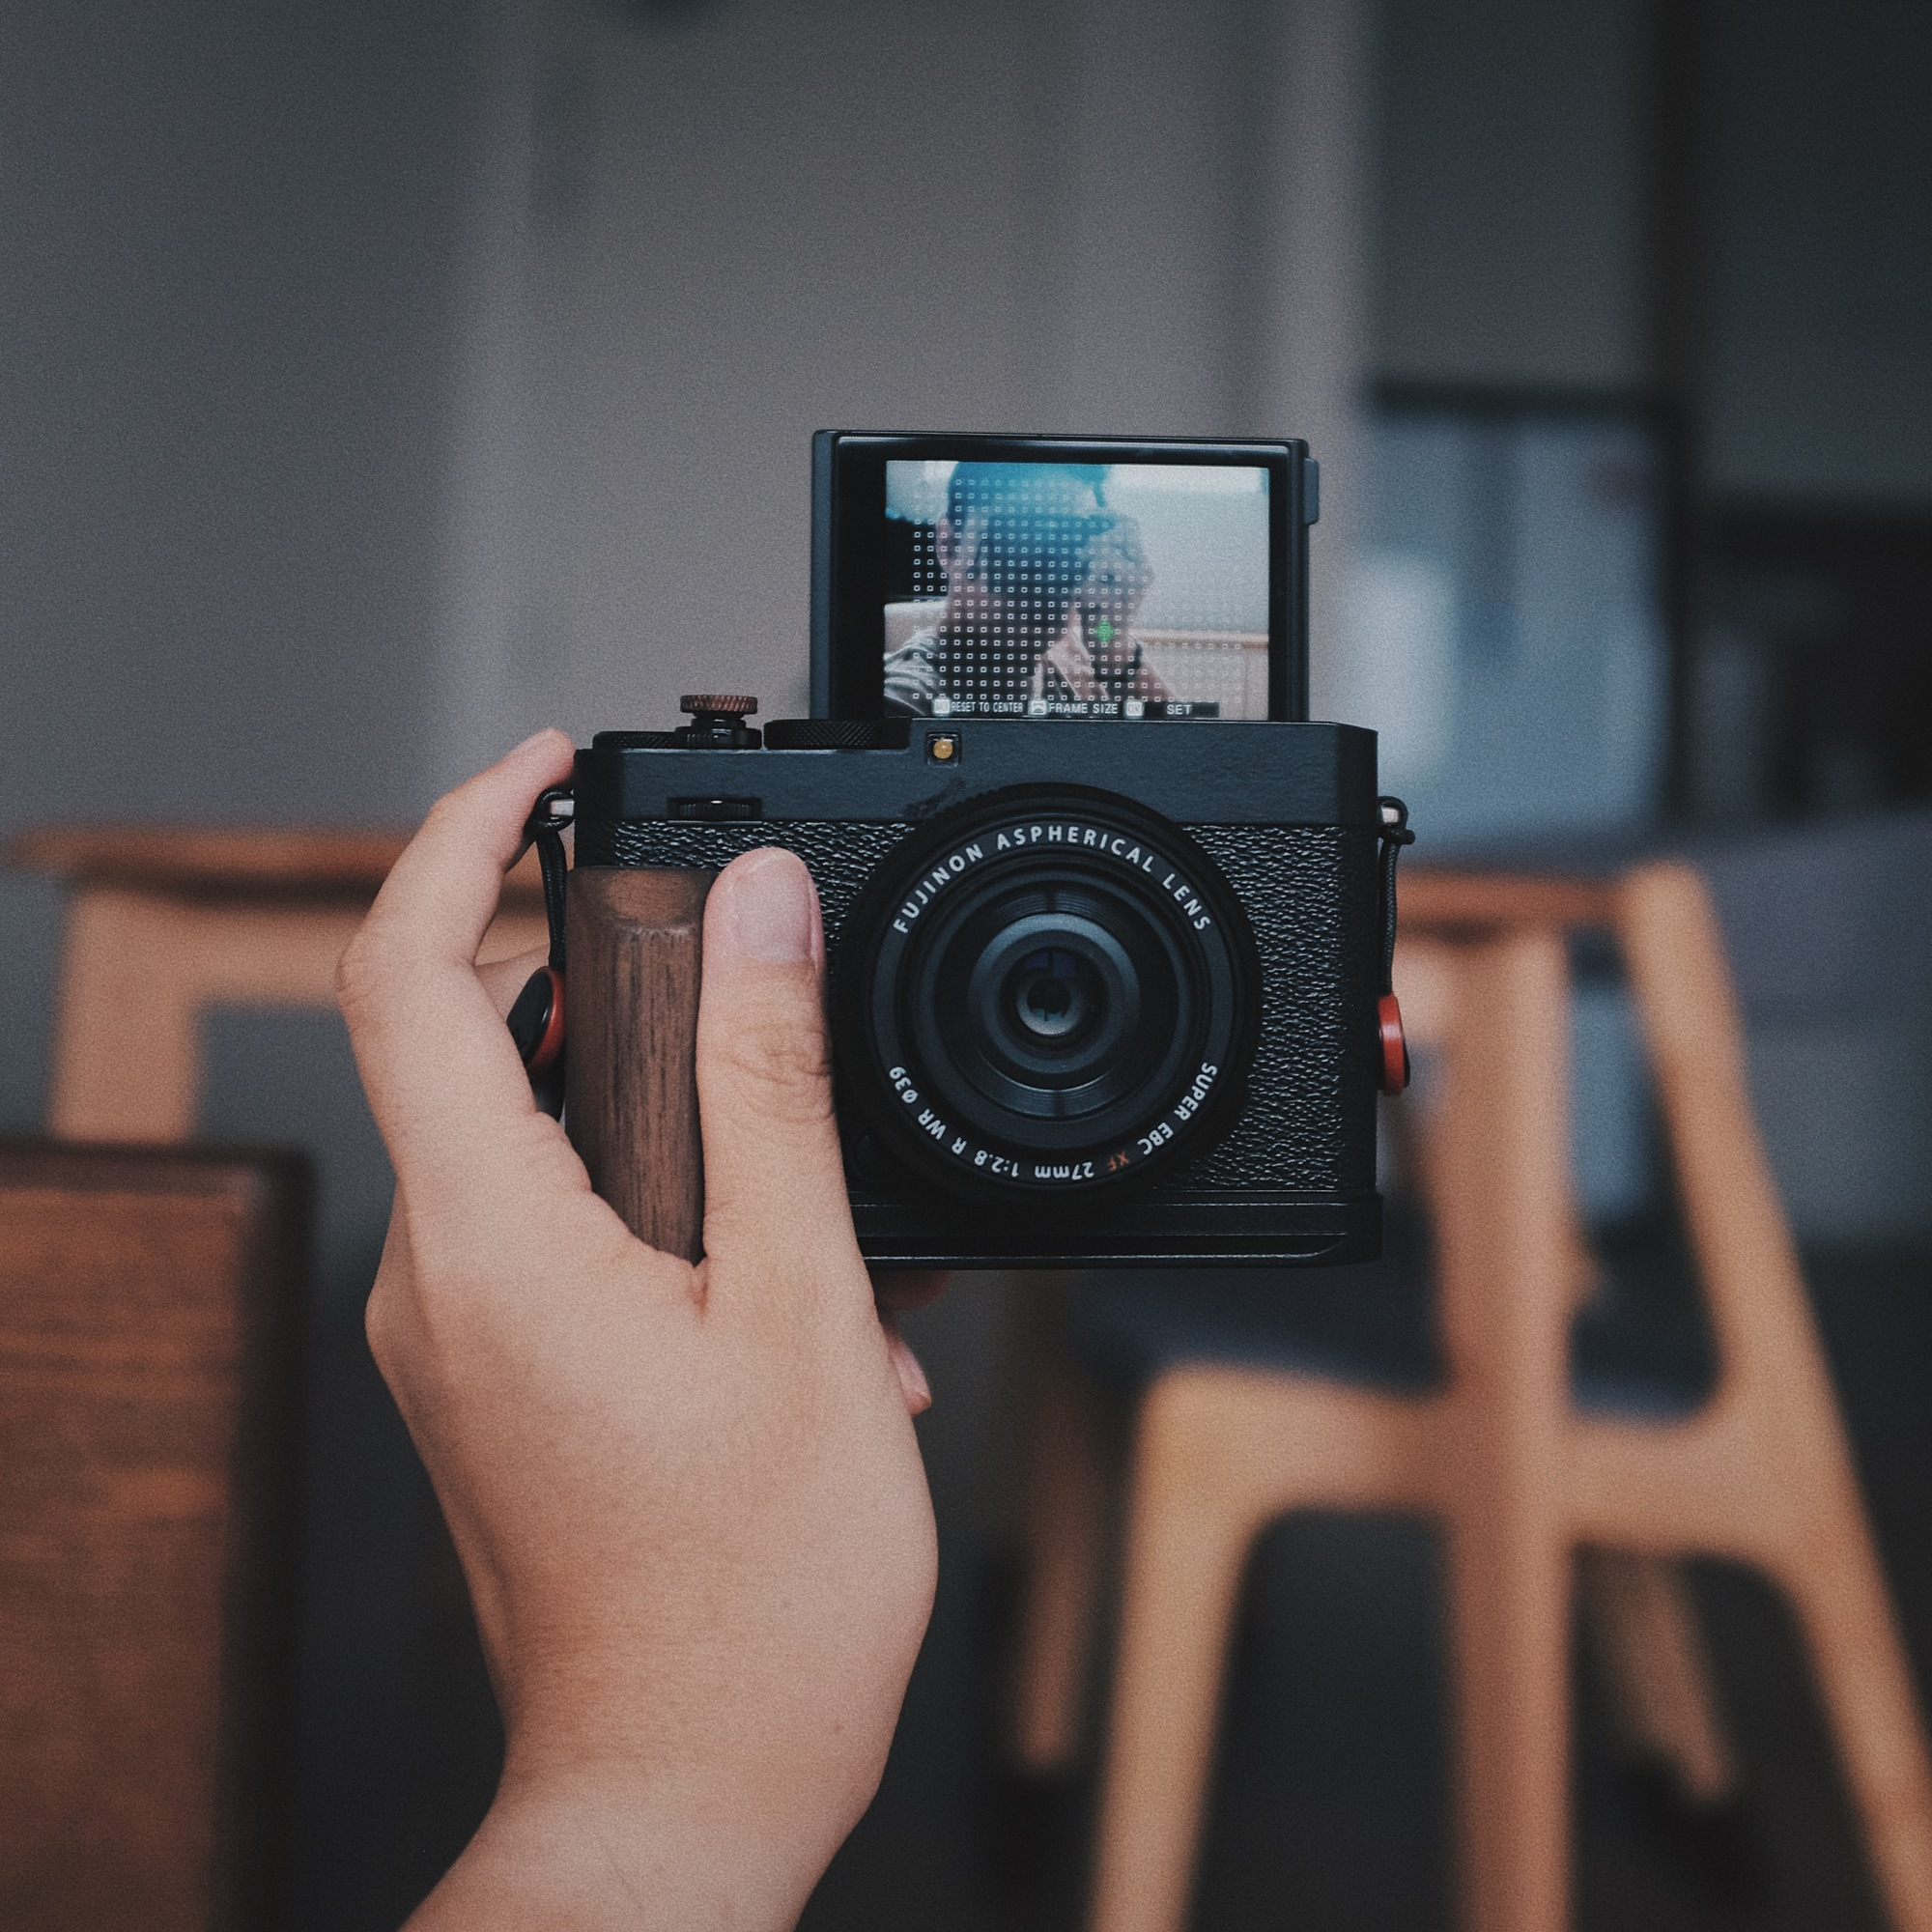
\includegraphics[width=\linewidth]{\envfinaldir/coverpic-prod.jpg}\par
            % \vskip 30pt
            \vfill

            \normalsize\rmfamily\scshape
            \copyright{} The Web Digest Project \hfill\large \envdatestr
        \end{center}
    \end{titlepage}
    % \restoregeometry
}
\newcommand{\simplehref}[1]{%
    \textcolor{blue!80!green}{\href{#1}{#1}}%
}
\renewcommand{\contentsname}{\center\Huge\sffamily\bfseries Contents\par\vskip 20pt}
\newcounter{ipartcounter}
\setcounter{ipartcounter}{0}
\newcommand{\ipart}[1]{
    % \vskip 20pt
    \clearpage
    \stepcounter{ipartcounter}
    \phantomsection
    \addcontentsline{toc}{chapter}{#1}
    % \begin{center}
    %     \Huge
    %     \sffamily\bfseries
    %     #1
    % \end{center}
    % \vskip 20pt plus 7pt
}
\newcounter{ichaptercounter}
\setcounter{ichaptercounter}{0}
\newcommand{\ichapter}[1]{
    % \vskip 20pt
    \clearpage
    \stepcounter{ichaptercounter}
    \phantomsection
    \addcontentsline{toc}{section}{\numberline{\arabic{ichaptercounter}}#1}
    \begin{center}
        \Huge
        \sffamily\bfseries
        #1
    \end{center}
    \vskip 20pt plus 7pt
}
\newcommand{\entrytitlefont}[1]{\subsection*{\raggedright\Large\sffamily\bfseries#1}}
\newcommand{\entryitemGeneric}[2]{
    % argv: title, url
    \parbox{\linewidth}{
        \entrytitlefont{#1}\par\vskip 5pt
        \footnotesize\ttfamily\mdseries
        \simplehref{#2}
    }\vskip 11pt plus 11pt minus 1pt
}
\newcommand{\entryitemGithub}[3]{
    % argv: title, url, desc
    \parbox{\linewidth}{
        \entrytitlefont{#1}\par\vskip 5pt
        \footnotesize\ttfamily\mdseries
        \simplehref{#2}\par\vskip 5pt
        \small\rmfamily\mdseries#3
    }\vskip 11pt plus 11pt minus 1pt
}
\newcommand{\entryitemAp}[3]{
    % argv: title, url, desc
    \parbox{\linewidth}{
        \entrytitlefont{#1}\par\vskip 5pt
        \footnotesize\ttfamily\mdseries
        \simplehref{#2}\par\vskip 5pt
        \small\rmfamily\mdseries#3
    }\vskip 11pt plus 11pt minus 1pt
}
\newcommand{\entryitemHackernews}[3]{
    % argv: title, hnurl, rawurl
    % \parbox{\linewidth}{
    %     \entrytitlefont{#1}\par\vskip 5pt
    %     \footnotesize\ttfamily\mdseries
    %     \simplehref{#3}\par
    %     \textcolor{black!50}{\href{#2}{#2}}
    % }\vskip 11pt plus 11pt minus 1pt
    \begin{minipage}{\linewidth}
            \entrytitlefont{#1}\par\vskip 5pt
            \footnotesize\ttfamily\mdseries
            \simplehref{#3}\par
            \textcolor{black!50}{\href{#2}{#2}}
    \end{minipage}\par\vskip 11pt plus 11pt minus 1pt
}







\begin{document}

\makeheader

\tableofcontents\clearpage




\ipart{Developers}
\ichapter{Hacker News}
\entryitemTwoLinks{Please don't force dark mode}{https://news.ycombinator.com/item?id=42762054}{https://iamvishnu.com/posts/please-dont-force-dark-mode}

\entryitemTwoLinks{Escape the walled garden and algorithm black boxes with RSS feeds}{https://news.ycombinator.com/item?id=42761219}{https://www.johnwalker.nl/posts/escape-the-walled-garden-with-rss}

\entryitemTwoLinks{Why is Git Autocorrect too fast for Formula One drivers?}{https://news.ycombinator.com/item?id=42760620}{https://blog.gitbutler.com/why-is-git-autocorrect-too-fast-for-formula-one-drivers/}

\entryitemTwoLinks{Using your Apple device as an access card in unsupported systems}{https://news.ycombinator.com/item?id=42759557}{https://github.com/kormax/apple-device-as-access-card}

\entryitemTwoLinks{TikTok says it is restoring service for U.S. users}{https://news.ycombinator.com/item?id=42759336}{https://www.nbcnews.com/tech/tech-news/tiktok-says-restoring-service-us-users-rcna188320}

\entryitemTwoLinks{Lenovo has removed the TrackPoint nub from new ThinkPad laptops}{https://news.ycombinator.com/item?id=42758570}{https://www.pcworld.com/article/2566195/lenovo-has-removed-its-iconic-trackpoint-nub-from-new-thinkpad-laptops.html}

\entryitemTwoLinks{Build a tiny CA for your homelab with a Raspberry Pi}{https://news.ycombinator.com/item?id=42758070}{https://smallstep.com/blog/build-a-tiny-ca-with-raspberry-pi-yubikey/}

\entryitemTwoLinks{The Fuzzing Book}{https://news.ycombinator.com/item?id=42756286}{https://www.fuzzingbook.org/}

\entryitemTwoLinks{``The Traitors'', a reality TV show, offers a useful economics lesson}{https://news.ycombinator.com/item?id=42755251}{https://www.economist.com/finance-and-economics/2025/01/16/the-traitors-a-reality-tv-show-offers-a-useful-economics-lesson}

\entryitemTwoLinks{About availability of TikTok and ByteDance Ltd. apps in the United States}{https://news.ycombinator.com/item?id=42754130}{https://support.apple.com/en-us/121596}

\entryitemTwoLinks{Haskell: A Great Procedural Language}{https://news.ycombinator.com/item?id=42754098}{https://entropicthoughts.com/haskell-procedural-programming}

\entryitemTwoLinks{The "35-cent" Commodore 64 softmodem}{https://news.ycombinator.com/item?id=42754057}{http://oldvcr.blogspot.com/2025/01/the-35-cent-commodore-64-softmodem.html}

\entryitemTwoLinks{Forgejo: A self-hosted lightweight software forge}{https://news.ycombinator.com/item?id=42753523}{https://forgejo.org/}

\entryitemTwoLinks{TikTok goes dark in the US}{https://news.ycombinator.com/item?id=42753396}{https://techcrunch.com/2025/01/18/tiktok-goes-dark-in-the-u-s/}

\entryitemTwoLinks{Yek: Serialize your code repo (or part of it) to feed into any LLM}{https://news.ycombinator.com/item?id=42753302}{https://github.com/bodo-run/yek}

\entryitemTwoLinks{We need to protect the protocol that runs Bluesky}{https://news.ycombinator.com/item?id=42752703}{https://www.technologyreview.com/2025/01/17/1110063/we-need-to-protect-the-protocol-that-runs-bluesky/}

\entryitemTwoLinks{How Unix spell ran in 64kb RAM}{https://news.ycombinator.com/item?id=42752604}{https://blog.codingconfessions.com/p/how-unix-spell-ran-in-64kb-ram}

\entryitemTwoLinks{Nation-scale Matrix deployments will fail using the community version of Synapse}{https://news.ycombinator.com/item?id=42752402}{https://mastodon.matrix.org/@element/113842786942364269}

\entryitemTwoLinks{Pharaoh's Tomb HD – A Remake Made in JavaScript with Kaplay}{https://news.ycombinator.com/item?id=42752023}{https://pt-hd.iocaihost.me/}

\entryitemTwoLinks{Kalman Filter Tutorial}{https://news.ycombinator.com/item?id=42751690}{https://www.kalmanfilter.net/default.aspx}\ichapter{Phoronix}
\entryitemGeneric{\hskip 0pt{}Linux To Allow Adjusting pid\_max Per PID Namespace - Helping Old Software}{https://www.phoronix.com/news/Linux-6.14-PID-Namespace}

\entryitemGeneric{\hskip 0pt{}A Last Minute Fix For EEVDF Scheduling Lag With Linux 6.13}{https://www.phoronix.com/news/Linux-6.13-Last-Minute-EEVDF}

\entryitemGeneric{\hskip 0pt{}Rust Coreutils 0.0.29 Brings Improved Compatibility, New Performance Optimizations}{https://www.phoronix.com/news/Rust-Coreutils-uutils-0.0.29}

\entryitemGeneric{\hskip 0pt{}Linux 6.14 EDAC Preps For Intel Clearwater Forest, Adds LoongArch Driver For ECC Memory}{https://www.phoronix.com/news/Linux-6.14-EDAC}

\entryitemGeneric{\hskip 0pt{}New "mountinfo" Program Set To Be Bundled With Linux 6.14}{https://www.phoronix.com/news/Linux-6.14-mountinfo}

\entryitemGeneric{\hskip 0pt{}QH Electronics Game Controller Support Being Added For Linux 6.14}{https://www.phoronix.com/news/QH-Electronics-XPad-Linux-6.14}

\entryitemGeneric{\hskip 0pt{}Linux 6.14 To Perform Better With The Drgn Debugger Via Faster /proc/kcore Reads}{https://www.phoronix.com/news/Linux-6.14-Faster-kcore-Reads}

\entryitemGeneric{\hskip 0pt{}GNU Debugger GDB 16.1 Brings Better Intel PT Support, gstack Added}{https://www.phoronix.com/news/GNU-Debugger-GDB-16.1}

\entryitemGeneric{\hskip 0pt{}Intel Tofino P4 Software Open-Sourced Years Later}{https://www.phoronix.com/news/Intel-Tofino-P4-Open-Source}\ichapter{Dribbble}
\entryitemGeneric{\hskip 0pt{}Wine Label}{https://dribbble.com/shots/25490604-Wine-Label}

\entryitemGeneric{\hskip 0pt{}planet}{https://dribbble.com/shots/25490310-planet}

\entryitemGeneric{\hskip 0pt{}Shihiko // E-commerce Website}{https://dribbble.com/shots/25489208-Shihiko-E-commerce-Website}

\entryitemGeneric{\hskip 0pt{}Wine Label}{https://dribbble.com/shots/25485370-Wine-Label}

\entryitemGeneric{\hskip 0pt{}EA System Ambigram}{https://dribbble.com/shots/25486215-EA-System-Ambigram}

\entryitemGeneric{\hskip 0pt{}Aquascaping Logos 🐠}{https://dribbble.com/shots/25486067-Aquascaping-Logos}

\entryitemGeneric{\hskip 0pt{}Puzzle Fintech Website Design}{https://dribbble.com/shots/25394559-Puzzle-Fintech-Website-Design}

\entryitemGeneric{\hskip 0pt{}Pemberton's Formula}{https://dribbble.com/shots/25480158-Pemberton-s-Formula}

\entryitemGeneric{\hskip 0pt{}RoundRobin 2.0}{https://dribbble.com/shots/25479558-RoundRobin-2-0}

\entryitemGeneric{\hskip 0pt{}Black Cats}{https://dribbble.com/shots/25478711-Black-Cats}

\entryitemGeneric{\hskip 0pt{}N\&R Social Media}{https://dribbble.com/shots/25159226-N-R-Social-Media}

\entryitemGeneric{\hskip 0pt{}Developing new skills}{https://dribbble.com/shots/25479409-Developing-new-skills}

\entryitemGeneric{\hskip 0pt{}Vertical Logos from the Portfolio}{https://dribbble.com/shots/25479968-Vertical-Logos-from-the-Portfolio}

\entryitemGeneric{\hskip 0pt{}Top 9 logos of 2024}{https://dribbble.com/shots/25479840-Top-9-logos-of-2024}

\entryitemGeneric{\hskip 0pt{}NEON Graphic Style}{https://dribbble.com/shots/25480590-NEON-Graphic-Style}

\entryitemGeneric{\hskip 0pt{}Gillespie Farms™}{https://dribbble.com/shots/25474556-Gillespie-Farms}

\entryitemGeneric{\hskip 0pt{}Document Scanner App}{https://dribbble.com/shots/25466972-Document-Scanner-App}

\entryitemGeneric{\hskip 0pt{}Faith Education Icons}{https://dribbble.com/shots/25422138-Faith-Education-Icons}

\entryitemGeneric{\hskip 0pt{}Round Robin}{https://dribbble.com/shots/25467606-Round-Robin}

\entryitemGeneric{\hskip 0pt{}Nexos crypto wallet}{https://dribbble.com/shots/25464532-Nexos-crypto-wallet}

\entryitemGeneric{\hskip 0pt{}Kraken Illustration}{https://dribbble.com/shots/25468020-Kraken-Illustration}

\entryitemGeneric{\hskip 0pt{}The best route to the corner office}{https://dribbble.com/shots/25468475-The-best-route-to-the-corner-office}

\entryitemGeneric{\hskip 0pt{}Glyph Beer 62}{https://dribbble.com/shots/25470954-Glyph-Beer-62}

\entryitemGeneric{\hskip 0pt{}B}{https://dribbble.com/shots/25466481-B}


\ipart{Developers~~~~(zh-Hans)}
\ichapter{Solidot}
\entryitemGeneric{\hskip 0pt{}手游 Marvel Snap 因 TikTok 禁令从应用商店下架}{https://www.solidot.org/story?sid=80372}

\entryitemGeneric{\hskip 0pt{}就业市场上的权力天平倾向了雇主}{https://www.solidot.org/story?sid=80371}

\entryitemGeneric{\hskip 0pt{}对 TikTok 的禁令可能扩散到美国盟国}{https://www.solidot.org/story?sid=80370}

\entryitemGeneric{\hskip 0pt{}TikTok 关闭美国服务}{https://www.solidot.org/story?sid=80369}

\entryitemGeneric{\hskip 0pt{}马斯克被发现雇佣游戏代练后恼羞成怒}{https://www.solidot.org/story?sid=80368}

\entryitemGeneric{\hskip 0pt{}原神被禁止向美国 16 岁以下儿童出售战利品箱}{https://www.solidot.org/story?sid=80367}

\entryitemGeneric{\hskip 0pt{}CNNIC 报告称中国有 2.49 亿人使用过生成式 AI}{https://www.solidot.org/story?sid=80366}

\entryitemGeneric{\hskip 0pt{}TikTok 在美最高法院败诉,准备周日关闭美国服务}{https://www.solidot.org/story?sid=80365}

\entryitemGeneric{\hskip 0pt{}科学家发现爱阅读的人的大脑与不爱阅读的人有差别}{https://www.solidot.org/story?sid=80364}

\entryitemGeneric{\hskip 0pt{}南方古猿的肉食量不大}{https://www.solidot.org/story?sid=80363}

\entryitemGeneric{\hskip 0pt{}考古学家在英国发现一个铁器时代的母系社会}{https://www.solidot.org/story?sid=80362}

\entryitemGeneric{\hskip 0pt{}Meta 朝通用翻译器前进了一大步}{https://www.solidot.org/story?sid=80361}

\entryitemGeneric{\hskip 0pt{}中国核电发电量到 2030 年将超越欧美}{https://www.solidot.org/story?sid=80360}

\entryitemGeneric{\hskip 0pt{}1984 年版《沙丘》导演大卫林奇去世}{https://www.solidot.org/story?sid=80359}

\entryitemGeneric{\hskip 0pt{}任天堂首席法务承认模拟器本身是合法的}{https://www.solidot.org/story?sid=80358}

\entryitemGeneric{\hskip 0pt{}小红书据报道可能切割中国用户和外国用户}{https://www.solidot.org/story?sid=80357}\ichapter{V2EX}
\entryitemGeneric{\hskip 0pt{}[分享创造] 《代码时光机》更新了一期汽车话题}{https://www.v2ex.com/t/1106324}

\entryitemGeneric{\hskip 0pt{}[问与答] 某书的这个怎么办}{https://www.v2ex.com/t/1106323}

\entryitemGeneric{\hskip 0pt{}[分享发现] 好东西 9.1 高分 真不错 推荐}{https://www.v2ex.com/t/1106321}

\entryitemGeneric{\hskip 0pt{}[站长] 请问大佬们:什么 CMS 可以做到类似这样的首页布局?}{https://www.v2ex.com/t/1106320}

\entryitemGeneric{\hskip 0pt{}[推广] 薅羊毛,港美股券商长桥富途老虎华盛开户邀请,渠道邀请奖励对半分}{https://www.v2ex.com/t/1106319}

\entryitemGeneric{\hskip 0pt{}[问与答] 官方固件的华硕路由器如何在重启后自动执行 iptables 命令?}{https://www.v2ex.com/t/1106318}

\entryitemGeneric{\hskip 0pt{}[Google] play store 购买闪退}{https://www.v2ex.com/t/1106316}

\entryitemGeneric{\hskip 0pt{}[分享发现] 小红书的翻译功能在被疯狂 hack}{https://www.v2ex.com/t/1106315}

\entryitemGeneric{\hskip 0pt{}[问与答] 这次川普发币事件会不会让风头完全被 ai 抢走的 web3 热一热?}{https://www.v2ex.com/t/1106314}

\entryitemGeneric{\hskip 0pt{}[程序员] 抹茶交易所 MEXC 在 KYC 的时候在闲鱼找的认证,提币封控}{https://www.v2ex.com/t/1106313}

\entryitemGeneric{\hskip 0pt{}[问与答] 码农的一生:人类的爱情到底是什么}{https://www.v2ex.com/t/1106312}

\entryitemGeneric{\hskip 0pt{}[分享创造] 36 岁本想做个独立开发,没成想润了出去}{https://www.v2ex.com/t/1106311}

\entryitemGeneric{\hskip 0pt{}[硬件] 英特尔 cpu i5 4200u,内存插槽支持多大的内存条呀?}{https://www.v2ex.com/t/1106310}

\entryitemGeneric{\hskip 0pt{}[问与答] 思考题 两点间的最短路径(测地线,也是光的传播路径)计算公式是什么?}{https://www.v2ex.com/t/1106309}

\entryitemGeneric{\hskip 0pt{}[YouTube] IDM 现在没法下载 youtube 了,还有啥其它好用的工具?}{https://www.v2ex.com/t/1106308}

\entryitemGeneric{\hskip 0pt{}[问与答] 大陆 app store 上架的话能接 openrouter 吗?}{https://www.v2ex.com/t/1106307}

\entryitemGeneric{\hskip 0pt{}[问与答] clash verge 做旁路由时,能指定某个设备用某个节点?}{https://www.v2ex.com/t/1106306}

\entryitemGeneric{\hskip 0pt{}[分享创造] [首批 10 名免费名额] 新年来临之际,给 V2EX 同胞送人工定制的视频贺卡福利。}{https://www.v2ex.com/t/1106305}

\entryitemGeneric{\hskip 0pt{}[问与答] 随着手机安卓 cpu 的改进, 是不是一般情况下,播放视频都不再需要使用 ffmpeg 之类的软件解码器了?}{https://www.v2ex.com/t/1106304}

\entryitemGeneric{\hskip 0pt{}[Surge] surge for iOS 找人}{https://www.v2ex.com/t/1106302}

\entryitemGeneric{\hskip 0pt{}[宽带症候群] 万能的 v 友可以租我一个欧洲-国内优化线路的 ts 服务器吗?}{https://www.v2ex.com/t/1106301}

\entryitemGeneric{\hskip 0pt{}[程序员] KDE Plasma 6.3 的小细节:鼠标拖拽文件,在松开鼠标按键前,所有窗口的位置覆盖状态保持不变}{https://www.v2ex.com/t/1106300}

\entryitemGeneric{\hskip 0pt{}[问与答] 沉溺于自我提升是不是走入了一种陷阱?}{https://www.v2ex.com/t/1106299}

\entryitemGeneric{\hskip 0pt{}[macOS] 有人需要 Setapp 年费订阅吗?¥ 260 元一 Mac 一 iOS}{https://www.v2ex.com/t/1106298}

\entryitemGeneric{\hskip 0pt{}[推广] [首批 10 名] 新年来临之际,给 V2EX 同胞送人工定制的视频贺卡福利。}{https://www.v2ex.com/t/1106297}

\entryitemGeneric{\hskip 0pt{}[宽带症候群] 發現 TATA 基本上對內地三網都不友好}{https://www.v2ex.com/t/1106296}

\entryitemGeneric{\hskip 0pt{}[职场话题] 职业规划,已经后悔}{https://www.v2ex.com/t/1106295}

\entryitemGeneric{\hskip 0pt{}[分享发现] 独立开发出海必备工具站!— 我的新产品}{https://www.v2ex.com/t/1106294}

\entryitemGeneric{\hskip 0pt{}[macOS] 新 mbp 从时间机器里恢复要好久啊}{https://www.v2ex.com/t/1106293}

\entryitemGeneric{\hskip 0pt{}[程序员] 这是饿了么的 BUG?还是有意为之}{https://www.v2ex.com/t/1106292}

\entryitemGeneric{\hskip 0pt{}[Ubuntu] ubuntu 用 vbetool dpms off 了再 on 后,显示乱码}{https://www.v2ex.com/t/1106291}

\entryitemGeneric{\hskip 0pt{}[YouTube] YouTube premium 清退,续费提示 We couldn't verify your country}{https://www.v2ex.com/t/1106289}

\entryitemGeneric{\hskip 0pt{}[Apple] 大家觉得在 macOS 和 iOS 上最缺什么类型的软件?}{https://www.v2ex.com/t/1106288}

\entryitemGeneric{\hskip 0pt{}[Android] 小米 HyperOS 不支持 1password 通行证密钥吗?}{https://www.v2ex.com/t/1106287}

\entryitemGeneric{\hskip 0pt{}[问与答] 前端项目\#埋点}{https://www.v2ex.com/t/1106286}

\entryitemGeneric{\hskip 0pt{}[程序员] 使用 AI 辅助创作 web3 项目}{https://www.v2ex.com/t/1106285}

\entryitemGeneric{\hskip 0pt{}[问与答] 感觉 8gen2 的安卓手机开饿了么美团抖音很卡,换骁龙 8E 能好点?}{https://www.v2ex.com/t/1106284}

\entryitemGeneric{\hskip 0pt{}[酷工作] [远程 Web3 交易所] 欢迎互联网背景 - 后端- Java x 1 , App-Flutter x 3 [Up to USD \$6,000 + 期权分红]}{https://www.v2ex.com/t/1106283}

\entryitemGeneric{\hskip 0pt{}[问与答] v 友有好的本地文本转语音的框架推荐吗,除了 ebook2audiobook}{https://www.v2ex.com/t/1106281}

\entryitemGeneric{\hskip 0pt{}[SSD] 三星 ssd T7 被 洗衣机折磨后,还能正常使用,奇迹~不知道可以用到什么时候}{https://www.v2ex.com/t/1106280}

\entryitemGeneric{\hskip 0pt{}[Google] 在某模拟器登录谷歌账号导致被封}{https://www.v2ex.com/t/1106279}

\entryitemGeneric{\hskip 0pt{}[微信] 微信关闭 VPN 代理后所有公众号文章图片无法打开,文字内容可以,如果是一个网络链接则无法打开,餐厅点餐扫码扫不出来,微信聊天正常,但消息推送有延迟,显示代理连接错误,微信是给我缓存了什么网络连接的配置吗?请问有遇到类似情况的吗,如何解决?}{https://www.v2ex.com/t/1106278}

\entryitemGeneric{\hskip 0pt{}[问与答] 咨询一个 Apple Watch 蜂窝版独立使用问题}{https://www.v2ex.com/t/1106277}

\entryitemGeneric{\hskip 0pt{}[职场话题] 新话题,如果周末协助完成了 xx 工作,要在周报上写上周末完成 xx 工作么?}{https://www.v2ex.com/t/1106276}

\entryitemGeneric{\hskip 0pt{}[程序员] 大学软件工程教的哪些什么流程图、E-R 图、工程图是不是实际完全用不上?换了好几家公司,小的、中的、大的都去过,从来都是开完会确认需求后就开发}{https://www.v2ex.com/t/1106274}

\entryitemGeneric{\hskip 0pt{}[前端开发] 前端面试 SVG}{https://www.v2ex.com/t/1106273}

\entryitemGeneric{\hskip 0pt{}[问与答] 恶心坏了,一加 7Pro 虚焊拿去维修后续}{https://www.v2ex.com/t/1106272}

\entryitemGeneric{\hskip 0pt{}[Apple] Mac 内网穿透到 Windows 远程桌面试验比较总结(向日葵、RustDesk、Tailscale/NetBird、frp)}{https://www.v2ex.com/t/1106271}

\entryitemGeneric{\hskip 0pt{}[问与答] IM 应用中更新前端数据的问题}{https://www.v2ex.com/t/1106270}

\entryitemGeneric{\hskip 0pt{}[Apple] 什么时候有商家开发一款国标三脚的 Mac 电源插头就好了}{https://www.v2ex.com/t/1106269}


\ipart{Generic News}







\clearpage
\leavevmode\vfill
\footnotesize

Copyright \copyright{} 2023-2025 Neruthes and other contributors.

This document is published with CC BY-NC-ND 4.0 license.

The entries listed in this newsletter may be copyrighted by their respective creators.

This newsletter is generated by the Web Digest project.

The newsletters are also delivered via Telegram channel \CJKunderline{\href{https://t.me/webdigestchannel}{https://t.me/webdigestchannel}}.\\
RSS feed is available at \CJKunderline{\href{https://webdigest.pages.dev/rss.xml}{https://webdigest.pages.dev/rss.xml}}.

This newsletter is available in PDF at
\CJKunderline{\href{https://webdigest.pages.dev/}{https://webdigest.pages.dev/}}.

The source code being used to generate this newsletter is available at\\
\CJKunderline{\href{https://github.com/neruthes/webdigest}{https://github.com/neruthes/webdigest}}.

This newsletter is also available in
\CJKunderline{\href{http://webdigest.pages.dev/readhtml/\envyear/WebDigest-20250120.html}{HTML}} and
\CJKunderline{\href{https://github.com/neruthes/webdigest/blob/master/markdown/\envyear/WebDigest-20250120.md}{Markdown}}.


\coverpic{https://unsplash.com/photos/a-large-room-with-a-wooden-floor-and-walls-nGNoK7BiPZ4}{Susan Q Yin}


\end{document}
